\documentclass[twocolumn]{article}
\usepackage{cite}
\usepackage{amsmath,amssymb,amsfonts}
\usepackage{algorithm}
\usepackage[noend]{algpseudocode}
\usepackage{graphicx}
\usepackage{textcomp}
\usepackage[margin=0.5in,footskip=0.25in]{geometry}
\usepackage[title]{appendix}
\usepackage{tabularx}
\usepackage{svg}

\title{Estimating and profiling missing housing and population data for Ireland}
\author{
    Seán Healy, Soren Dreano\\
    \texttt{\{healys47,soren.dreano2\}@mail.dcu.ie}
    \footnote{This work was completed as part of the CA-660 module.}
}

\def\justifying{%
  \rightskip=0pt
  \spaceskip=0pt
  \xspaceskip=0pt
  \relax
}

\begin{document}

\maketitle
\begin{abstract}
This work models missing historical and projection data for Irish
housing and population on the county level, using available
property price, rent price and population data.  Analysis was
carried out in order to determine statistical correlates.  Then linear
regression was used for the purpose of determining missing historical property
prices, missing population projections, and missing historical rent prices,
all on the county level.  Finally, for visualisation purposes, county rent
profiles were produced using a clustering technique.
\end{abstract}\\\\
{\bf Keywords:} accommodation, housing, population, rent

\section{Introduction\label{s:intro}}
The CSO provide a very extensive collection of data sets at
{\tt data.cso.ie}.  These data cover rent and property price, population
records, estimates and projections.

Despite the broad array of datasets, it remains difficult to statistically
compare variables, since the datasets tend to vary in geographic granularity,
interval granularity, and overall timespan.

In ascending order of size, the geographic granularities (or \underline{zone type}) are {\bf eircode prefix},
{\bf sub-county} (e.g. Dublin 2 or Fingal), {\bf city}, {\bf county}, {\bf province}, {\bf region} and {\bf state}.  Online resources provide a mapping of
these granularities to each other, e.g. eircodes are mapped within counties via crowdsourcing
\cite{eircode19}, as listed in Appendix \ref{a:eircode}.  Counties are then mapped to geographic
regions by the CSO itself \cite{cso_regions}.  The remaining {\bf state} level is an aggregate of variables
across the entire Republic of Ireland.

Alongside this array of geographic granularities, there are a number of interval granularities used by CSO
datasets.  Some sets use {\bf monthly} datapoints, others use {\bf quarterly}, {\bf biannual}, {\bf annual}
or {\bf sparsely annual}.  Census data is generally sparsely annual, for example, since there are only
censuses every few years.

Granularity is not the only incompatibility across data sources from the CSO.
The overall timespan for data sets vary greatly.  Population records are split
across multiple data sets, some dating as far back as 1841.  By contrast,
county population for 2006 is only released under a standalone dataset.  Some
rent data is released between the years 2008 and 2021, whereas county-level
property price records only begin in 2010.

After aggregation is applied to datasets, rendering them compatible, linear
regression can be used to estimate missing data when a strongly correlated
variable is present.  Then a third issue arises: information overload.  Much of
the counties near Donegal, for example, follow similar trends for rent.  This
makes data difficult to visualise and reason about.  For this, ``rent
profiles'' can be created via clustering.  Finally, rent, population and
property prices can be compared across these few profiles rather than across
the overly granular county-levels, or the overly geographic CSO regional
level.

The issues that this work attempts to address can be summarised under three headings,
which are explained across sections \ref{ss:aggregation} to
\ref{ss:profiling}.

\section{Methodology}
\subsection{Aggregation and interpolation\label{ss:aggregation}}
Other than the regional and eircode mappings, which were compiled by hand from
online sources \cite{eircode19, cso_regions}, all data were downloaded via the
{\tt data.cso.ie} website, and preprocessed to remove out-of-scope data.  A listing of
the CSO data source IDs, and what purpose they were used for in this work, may
be found in Appendix \ref{a:sources}.

As suggested in Section \ref{s:intro}, most data sources differed in granularity
and timespan.

\begin{table}[h!]
\centering
\begin{tabularx}{0.5\textwidth}{r X X X X X}
    \textit{Source} & \textit{Interval} & \textit{Zone type} & \textit{Begins} & \textit{Ends} \\ \hline
    E2004 & Sparse & County, city & 2011 & 2014 \\ \hline
    C0103 & Sparse & Various & 2006 & 2006 \\ \hline
    B0102 & Sparse & Various & 1841 & 2002 \\ \hline
    PEC08 & Sparse & Various & 2011 & 2046 \\ \hline
    RIH02 & Biannual & Various & 2006 & 2021 \\ \hline
    HPM04 & Monthly & Eircode prefix & 2010 & 2021 \\ \hline
    HPM09 & Monthly & Various & 2005 & 2021 \\ \hline
    CIA02 & Annual & Region, county & 2000 & 2018 \\ \hline
    BHA12 & Annual & Region, county & 1975 & 2020 \\ \hline
    HSA09 & Annual & State & 1975 & 2016 \\ \hline
    BBM02 & Monthly & State & 1975 & 2008 \\ \hline
    PEA18 & Annual & State & 1987 & 2021
\end{tabularx} \\
\caption{Data sources considered or used in this work}
\label{tab:sources}
\end{table}

When there were various zone types present in a data source (e.g. state, province
and county), much of the data was filtered so that only one zone type remained,
ideally county data.  To aggregate sum data, a simple sum of constituents was used.
E.g. the total volume of house sales in a county is the same as the sum of volumes
for that counties' constituent eircode prefixes.

Mean data was aggregated using a weighted mean.  E.g. the mean property price in
Louth is the volume-weighted mean of the house prices in eircode prefixes
A91 and A92 (Laois' only eircode prefixes).  This ensures an eircode with very little
sale volume does not have a disproportionate effect on the aggregated mean for the
larger surrounding region.

For pre-processing data into less granular intervals, a similar aggregating approach
was used.  Turning monthly sum data into annual sum data involves summing all the months'
data points.  In contrast, turning monthly mean data into annual mean data involves taking a weighted
mean of the monthly data.  E.g. in (\ref{eq:weighted_mean}) the mean annual property
$\mu_{\text{price}}(y)$ can be determined by iterating through each month $m$ in
year $y$, summing the product of the month's mean price $\mu_{\text{price}}(m)$ and the month's total volume
$v(m)$.  That entire sum is divided by the year's total volume $v(y)$, producing the
year's mean property price.

\begin{align}
    \mu_{\text{price}}(y) = \frac{\sum^{m \in M(y)}\mu_{\text{price}}(m) \times v(m)}
    {v(y)}\label{eq:weighted_mean}
\end{align}

Interpolation was used to convert from sparse to dense data.  Census data
is only available every few years, so in this work, linear interpolation was
used to estimate population on state, county and region levels between any two
given years, e.g for the 4 missing years between the 2011 and 2016 censuses.
Unlike aggregation, which produces an
exact, known value, interpolation introduces uncertainty, because the
interpolated data points are only estimates.  It was noted early on in this
work that Irish population tends to move slowly and smoothly, so we chose
linear interpolation to find missing points between known points, and accepted
the inaccuracy of the estimates as negligible.

Interpolation isn't to be confused with the techniques that will be discussed in
Section \ref{ss:estimating}, where instead, two variables are considered, one known
and another unknown.  Interpolation uses one variable, and can only estimate points between
two known points, i.e. nothing before the first or after the last point.

\subsection{Estimating missing data\label{ss:estimating}}
As mentioned in Section \ref{s:intro}, linear regression was chosen as a candidate for
estimating missing data points.  For this to work, however, a strong correlation must first
be found between two or more variables.  Section \ref{ss:aggregation} laid the foundation
for comparison of different variables; instead of several incompatible tables, this section assumes
pre-processed tables, where the interval granularity is \underline{annual}, the zone type is
mostly \underline{county}, and missing years have been interpolated into usable data points.

County-level population projections were obtained by leveraging
regression to estimate county-regional population proportions as a function of
time, then combining the resulting estimates with CSO-published regional population
projections.

CSO presently only offers population projections for the broad
regions outlined in Appendix \ref{a:regions}.  However, it's possible to
estimate the population projections for the counties that comprise these
regions by splitting each region's projection in an uneven manner that
reflects the population proportions counties hold in each region.  Dublin is its
own standalone CSO region, so no action was required in that case.  However, in
the case of CSO's Midlands region, for example, the population projections for the counties
within that region could be estimated by splitting the regional estimate.

A naive approach to regional-to-county population projection conversion would
assume that the proportion of a region's population that a particular county
covers remains constant; if a region with only two counties, $A$ and $B$, has a
population ratio of $1:2$ between those two counties in 2021, the naive
assumption would be that those counties would display the same ratio in 2036.
However, it is observed that counties can become more or less prominent
portions of their regions as time goes on.  This is evident in Figure
\ref{midlands}.  Laois used to be the most populous county in the Midlands, but
now Westmeath is, and Longford has become significantly less proportional in
that region over the past century.

\begin{figure}
    \centering
    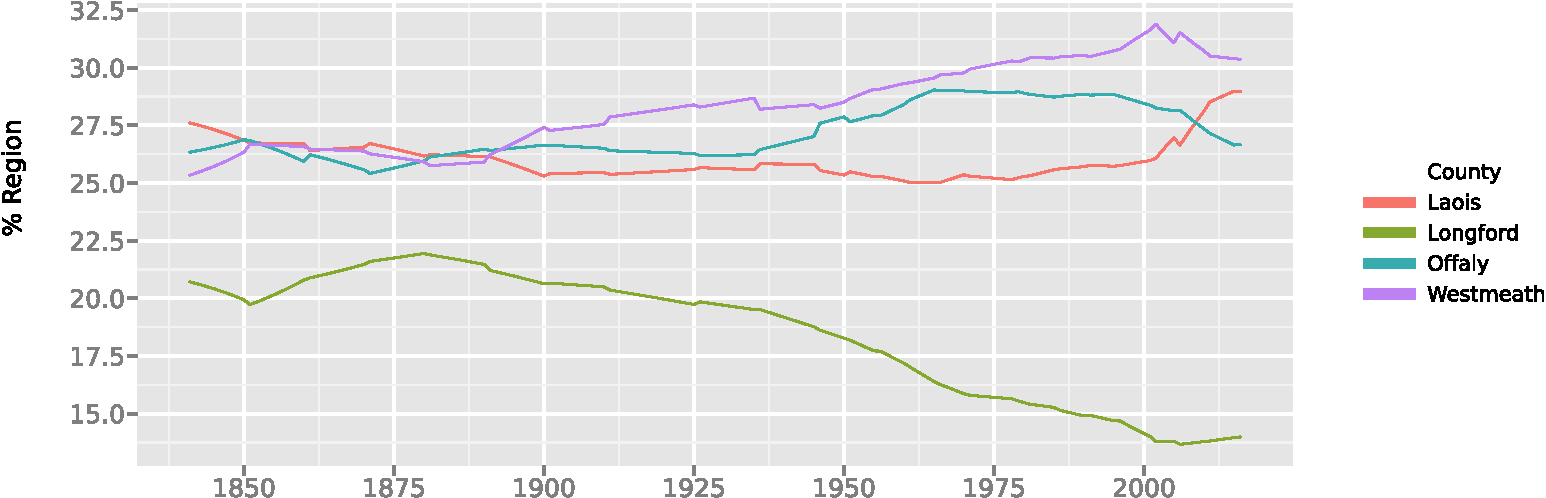
\includegraphics[width=0.55\textwidth]{media/pdf/midlands-population-proportion.svg.pdf}
    \caption{Distribution of population in the Midlands region\label{midlands}}
\end{figure}

Using data from Figure \ref{midlands}, lines are fitted over the county plots in
order to predict what regional proportion a county will comprise further
into the future (e.g. in 2036).  These lines are also normalised at each time
interval (each year), so that the county proportions for each region sum to 1.0
at each interval.

When these predicted proportions are multiplied by the
regional predictions, estimates for county populations are obtained.  Figure
\ref{regression1} illustrates the efficacy of this model.  The figure uses the
model to
produce estimations of pre-2017 population, which can then be compared against
the known or interpolated populations for those counties at given years.

\begin{align}
    & p(y, c) = p(y, r(c)) \times \frac{p(y, c)}{p(y, r(c))}
    \label{eq:pop_model_deriv} \\
    & \hat{p}(y, c) = p(y, r(c)) \times \hat{q}(y, c)
    \label{eq:pop_model}
\end{align}

The formula representing this regression technique is derived from
(\ref{eq:pop_model_deriv}).  Here, $p(y, c)$ means {\it the population of}
county $c$ in year $y$.  $r(c)$ returns the broader region of county $c$;
e.g. $r(\text{`Donegal'}) = \text{`Border'}$.  The observation (\ref{eq:pop_model_deriv}) has one particular part, $\frac{p(y, c)}{p(y, r(c))}$, for which
an estimate $\hat{q}(y, c)$ has previously been suggested.  $\hat{q}(y, c)$ is defined as the
predicted proportion of the outer region a county $c$ fills during year $y$.
E.g. 
$\hat{q}(2017, \text{`Westmeath'}) \approx 30\%$, and 
$\hat{q}(2036, \text{`Westmeath'}) \approx 33\%$.  This can be described
in terms of {\it Westmeath becoming increasingly populous within the context
of its Midlands region}.
Finally, (\ref{eq:pop_model_deriv}) leads to a model (\ref{eq:pop_model})
for estimating county population when only regional population predictions
and historical county population records exist.

\begin{figure}
    \centering
    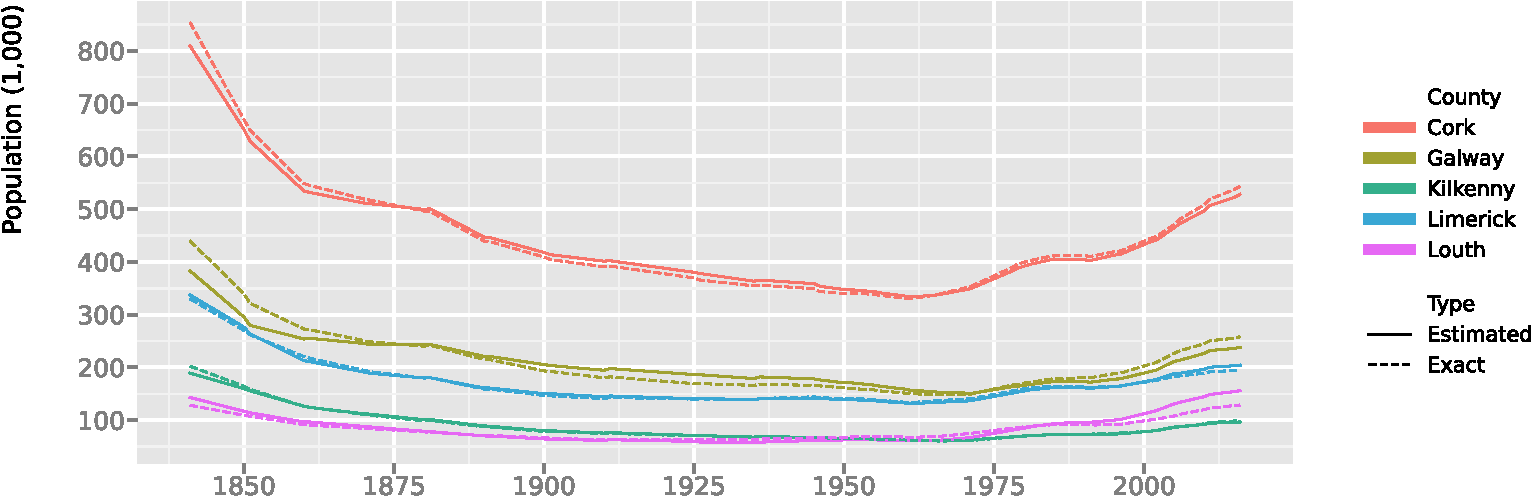
\includegraphics[width=0.48\textwidth]{media/pdf/population_by_county_linear_regression.svg.pdf}
    \caption{Regression county population estimation\label{regression1}}
\end{figure}

Regression was also used to estimate missing
historical data for house prices.  CSO publishes property price data in two
ways: firstly a historical price `index', and secondly, exact sale volumes and
mean prices.  The problem is the former data source is broader in time range
the latter.  Mean price data is missing before 2010, whereas the index data
goes as far back as 2005.  From a research perspective, it would be useful to
obtain estimated house price data that spans before the 2008 recession.

After verifying that the index does indeed correlate with the
price data during overlapping years, linear regression was used to extend
estimated mean property price data back to 2006.  One linear regression pass
per county was used, as illustrated in Figure (\ref{per_county}).

\begin{figure}
    \centering
    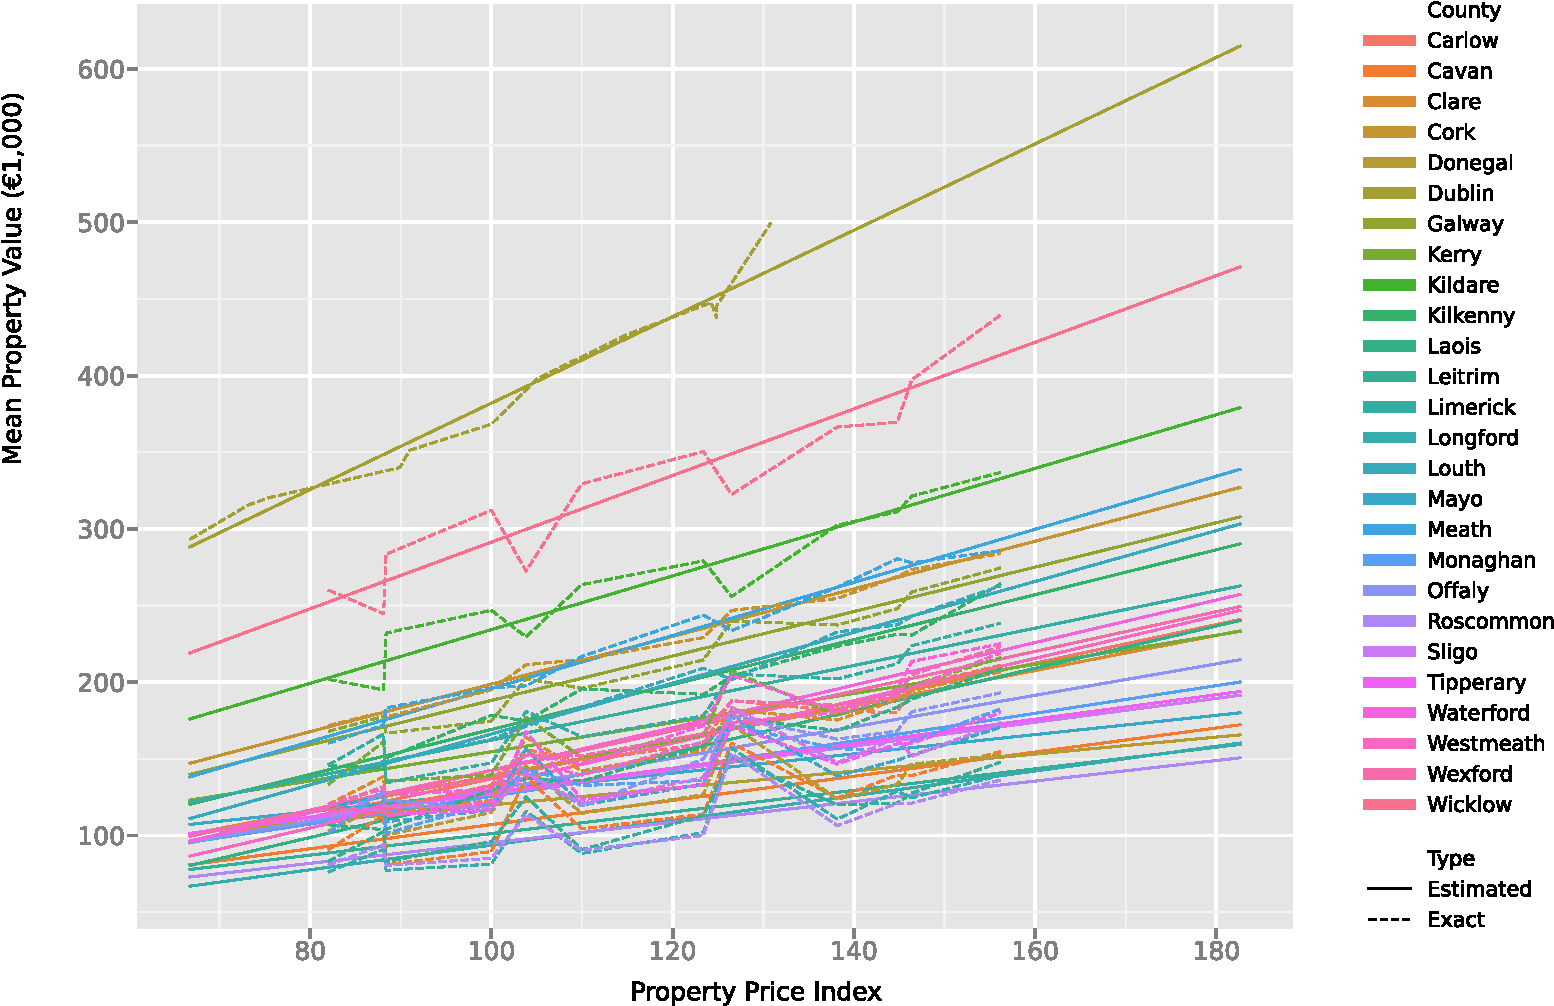
\includegraphics[width=0.50\textwidth]{media/pdf/property_price_linear_regression.svg.pdf}
    \caption{Estimating mean property price using linear regression over CSO price indices\label{per_county}}
\end{figure}

\subsection{Profiling\label{ss:profiling}}

After using linear regression to estimate missing data (both in the past
and future), a problem of information overload became more apparent.
Some counties correlated so closely in terms of rent prices that any study
of rent in Ireland would benefit from forming {\it profiles} or {\it county
groups}.  A form of hierarchical clustering was used to group counties
into 5 profiles based on historical rent prices.  The heuristic used was
{\it lowest difference between rent as a function of time}, $\Delta(g_1, g_2)$.
This approach is outlined in Algorithm \ref{cluster},  which takes a set of
counties $C$ as input, along with a desired number of rent profiles, $k$.  The
counties are first converted to singleton profiles $\{c\} \in K$.  At
initialisation $|K| = |C|$, but each round, a profile $g_1$ is merged with
another, $g_2$, according to minimum difference
($argmin_{\{g_1, g_2\} \subset K}\Delta(g_1, f_2)$), reducing the cardinality
of $|K|$ by one.  This repeats until we are left with the desired $k$ rent
profiles.

\begin{algorithm}
\caption{Clustering counties by rent similarity\label{cluster}}
\begin{algorithmic}[1]
    \State Input: $C$, $k$
    \State $K \leftarrow \{\{c\} \mid c \in C\}$
    \While{$|K| > k$}
    \State \{$g_1, g_2\} \leftarrow argmin_{\{g_1, g_2\} \subset K}\Delta(g_1, g_2)$
    \State $K \leftarrow (K - \{g_1, g_2\}) \cup \{g_1 \cup g_2\}$
    \EndWhile
\end{algorithmic}
\end{algorithm}

\section{Results}

As illustrated in Figure \ref{rent_groups}, the resulting rent profiles from
Algorithm \ref{cluster} depart from the standard geographic regions used by the
CSO.  These profiles (outlined in Table \ref{rent_group_tab}).  may provide a
better lens for comparison of rent progression and property price progression
going forward.

\begin{table}[h!]
\centering
\raggedright
\begin{tabularx}{0.5\textwidth}{r l l}
    \textit{Group} & \textit{Rent} & \textit{Counties} \\ \hline
    1 & Low & Cavan, Roscommon, Donegal,\\&&Longford, Leitrim, Mayo, Tipperary \\ \hline
    2 & Medium-low & Carlow, Kilkenny, Clare, Kerry,\\&&Wexford, Waterford, Offaly, Sligo,\\&&Laois, Westmeath \\ \hline
    3 & Medium & Cork, Galway, Meath, Limerick,\\&&Louth \\ \hline
    4 & Medium-high & Kildare, Wicklow \\ \hline
    5 & High & Dublin
\end{tabularx} \\
\justifying
\caption{Rent groups\label{rent_group_tab}}
\label{tab:sources}
\end{table}

\begin{figure}[H]
    \centering
    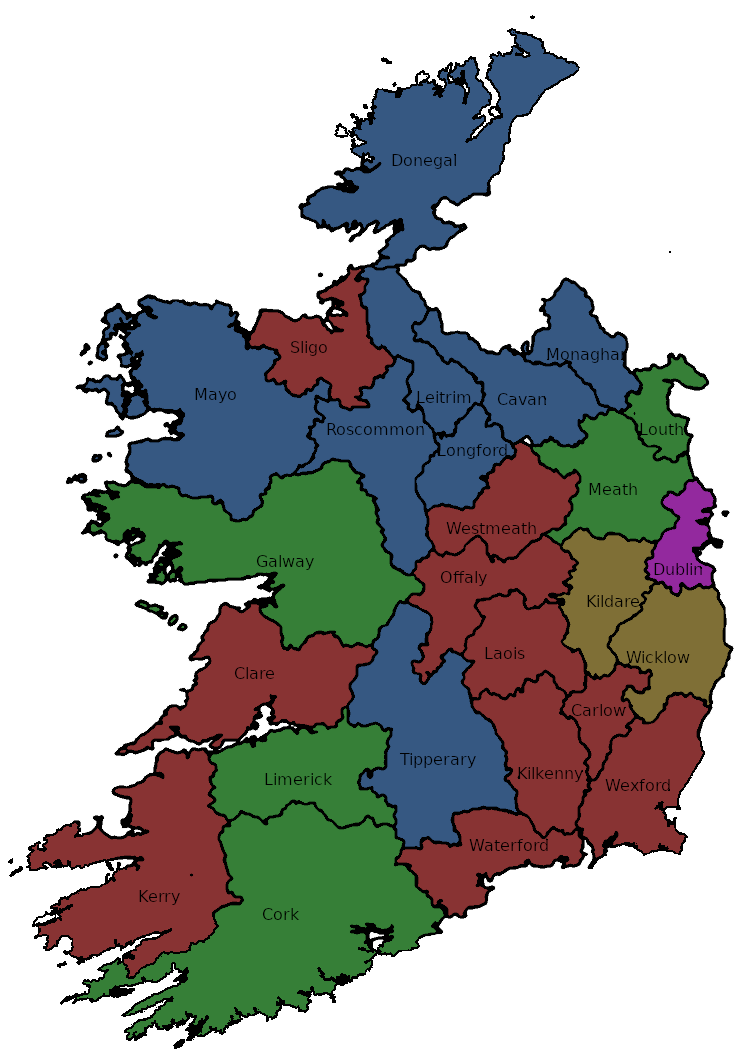
\includegraphics[width=0.25\textwidth]{media/clustered_ireland_map.png}
    \caption{Rent profiles\label{rent_groups}}
\end{figure}

\begin{figure}[h]
    \centering
    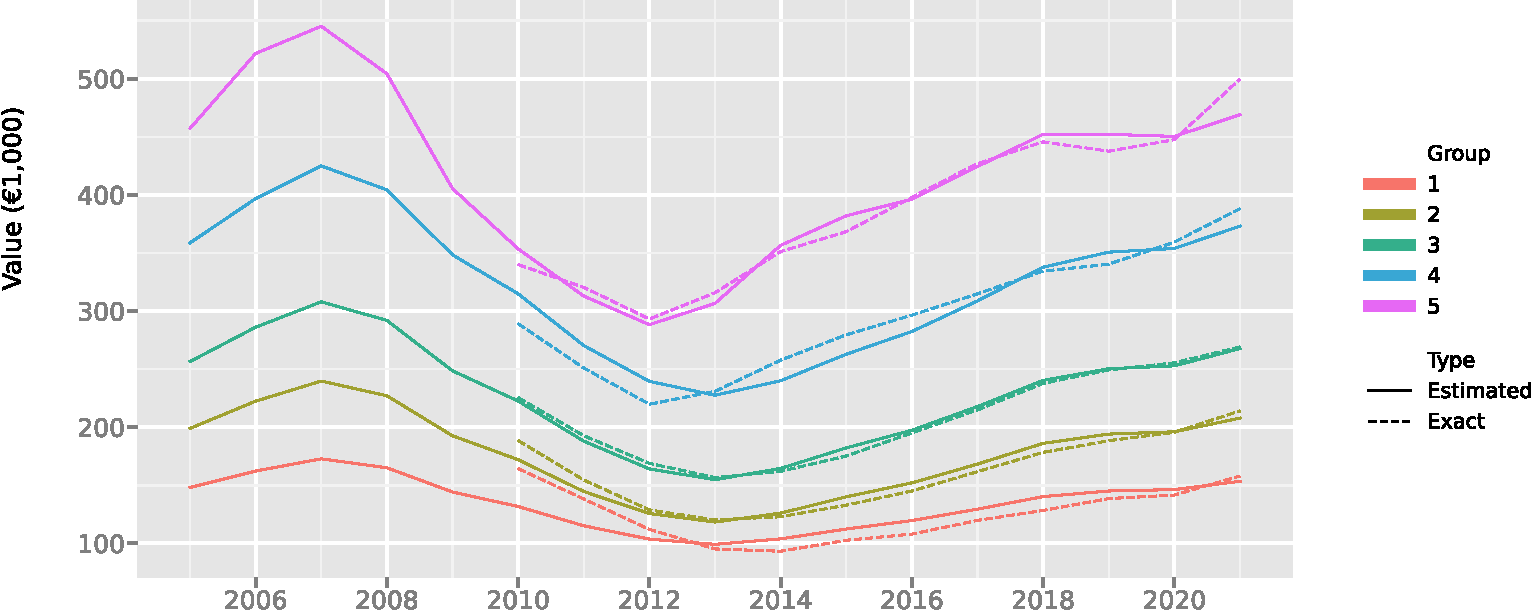
\includegraphics[width=0.505\textwidth]{media/pdf/estimated_property_value_by_county_group.svg.pdf}
    \caption{A fuller picture of property prices in Ireland \label{full_pic}}
\end{figure}

These profiles were used to produce the historical property price plot in
Figure \ref{full_pic}, which also includes estimated property prices
resulting from the methods outlined in Section \ref{ss:estimating}.

\section{Discussion\label{s:discuss}}

\subsection{Property price}
Unsurprisingly, the mean price to buy a property decreased from 2010 to 2012
after the Irish Property Bubble collapsed. The price surged drastically in most
counties and most notably in Dublin, Kildare, Wicklow, Cork and Galway. This
trend is shown clearly in figure 2. \begin{center}
\begin{tabular}{||c c||}
 \hline
 County & Increase in property price (\%) \\ [0.5ex]
 \hline\hline
 Dublin & 36.53 \\
 \hline
 Kildare & 36.49 \\
 \hline
 Wicklow & 34.43 \\
 \hline
 Cork & 20.37 \\
 \hline
 Galway & 11.44 \\ [1ex]
 \hline
\end{tabular}
\end{center}

\subsection{Rent price}
As shown in figure 3, the same pattern applies for the average renting price. Figure 4 presents a tight correlation between the evolution of both property price and rent cost.

\section{Factors}
\subsection{Population}
The increase in inhabitants might drive prices in the housing market up, as
there will be more demand for the same number of accommodation. In order to
test this theory, we looked at correlations between the total population of a
county and the mean property price, from 2010 to 2016, for each county. Figure
6 is a kernel density estimation of the correlation and shows how much this
correlation varies from county to county, with the mean being 0.309 and the
standard deviation 0.369.

The Donegal, Leitrim, Roscommon, Sligo and Tipperary counties actually have a
negative correlation between property price and population.

The property prices decreased while the population continued to increase in all of the aforementioned counties.

\begin{center}
\begin{tabular}{||c c c c||}
 \hline
 County & Pop. 2016 & Pop. 2010 & Evolution \\ [0.5ex]
 \hline\hline
 Donegal & 159192 & 157748 & 1444 \\
 \hline
 Leitrim & 32044 & 30934 & 1110 \\
 \hline
 Roscommon & 64544 & 62248 & 2296 \\
 \hline
 Sligo & 65535 & 64378 & 1157 \\
 \hline
 Tipperary & 159553 & 155268 & 4285 \\ [1ex]
 \hline
\end{tabular}
\end{center}

In the later part of the Celtic Tiger, a term referring to the economy of Ireland from the mid 1990s to the late 2000s, the Irish Property Bubble started to appear, which manifested itself as a constant and continuous rise in prices for almost a decade. In September 2008, the Irish government officially acknowledged the country's descent into recession\cite{kollewe08}, the collapse of the previously mentioned bubble being one of the major contributing factor to the global 2008 financial crisis. Unemployment rate rose from 6.5\% in July 2008 to 14.8\% 4 years later \cite{cso14} and house prices fell from 35\% between the end of 2007 and the end of 2010 \cite{environ10}.

Concerns around property prices began to rise a few years later, in mid-2012, as seen is figure 1, the number of queries on the Google search engine for the term "Property price" started surging in this period and costs continue escalating in Ireland \cite{kennedy21}.

\section{Conclusion}
The current Tánaiste Leo Varadkar recently said "One of our biggest deficiencies, in housing supply in Ireland, is we're a country of three-bed homes by-and-large and we don't have enough one-bed homes" \cite{mcgrath21}. We could not find any publicly available data on the matter. Nonetheless, an analysis on the housing supply in Ireland either by size or the number of bedrooms, especially in dense urban areas such as Dublin, Cork or Galway might confirm this deficiency. Further research should focus on the types of housing that sell the most and that have been constructed recently.

%[5]Central Statistics Office, <https://data.cso.ie/>
%[6]https://github.com/Gailenstorm/CA-660

\bibliographystyle{IEEEtran}
\raggedright
\bibliography{references}
\appendix
\section{Eircode Prefixes\label{a:eircode}}
\begin{tabularx}{0.5\textwidth}{r X}
    \textit{County} & \textit{Eircode Prefix} \\ \hline
    Carlow & R21, R93 \\ \hline
    Cavan & H12, H14, H16 \\ \hline
    Clare & V14, V15, V95 \\ \hline
    Cork & P12, P14, P17, P24, P25, P31, P32, P36, P43, P47, P51, P56, P61, P67, P72, P75, P81, P85, T12, T23, T34, T45, T56 \\ \hline
    Donegal & F92, F93, F94 \\ \hline
    Dublin & A41, A42, A45, A94, A96, D01, D02, D03, D04, D05, D06, D6W D07, D08, D09, D10, D11, D12, D13, D14, D15, D16, D17, D18, D20, D22, D24, K32, K34, K36, K45, K56, K67, K78 \\ \hline
    Galway & H53, H54, H62, H65, H71, H91 \\ \hline
    Kerry & V23, V31, V92, V93 \\ \hline
    Kildare & R14, R51, R56, W12, W23, W34, W91 \\ \hline
    Kilkenny & R95 \\ \hline
    Laois & R32 \\ \hline
    Leitrim & N41 \\ \hline
    Limerick & V35, V42, V94 \\ \hline
    Longford & N39 \\ \hline
    Louth & A91, A92 \\ \hline
    Mayo & F12, F23, F26, F28, F31, F35 \\ \hline
    Meath & A82, A83, A84, A85, A86, C15 \\ \hline
    Monaghan & A75, A81, H18, H23 \\ \hline
    Offaly & R35, R42, R45 \\ \hline
    Roscommon & F42, F45, F52 \\ \hline
    Sligo & F56, F91 \\ \hline
    Tipperary & E21, E25, E32, E34, E41, E45, E53, E91 \\ \hline
    Waterford & X35, X42, X91 \\ \hline
    Westmeath & N37, N91 \\ \hline
    Wexford & Y21, Y25, Y34, Y35 \\ \hline
    Wicklow & A63, A67, A98, Y14
\end{tabularx}
\section{CSO Regions\label{a:regions}}
\begin{tabularx}{0.5\textwidth}{r X}
    \textit{Region} & \textit{Counties} \\ \hline
    Border & Donegal, Sligo, Leitrim, Cavan, Monaghan\\ \hline
    Dublin & Dublin\\ \hline
    Mid-East & Wicklow, Kildare, Meath, Louth\\ \hline
    Midlands & Longford, Westmeath, Offaly, Laois\\ \hline
    Mid-West & Clare, Tipperary, Limerick\\ \hline
    South-East & Waterford, Kilkenny, Carlow, Wexford\\ \hline
    South-West & Cork, Kerry\\ \hline
    West & Galway, Mayo, Roscommon
\end{tabularx}
\section{CSO Data Sources\label{a:sources}}
\begin{tabularx}{0.5\textwidth}{r X}
    \textit{Region} & \textit{Counties} \\ \hline
    Population & E2004, C0103, B0102 \\ \hline
    Population projection & PEC08 \\ \hline
    Rent & RIH02 \\ \hline
    Property price & HPM04  \\ \hline
    Estimated property price & HPM09 \\ \hline
    Income data & CIA02 \\ \hline
    Planning permission data & BHA12 \\ \hline
    Construction cost data & HSA09 \\ \hline
    Construction employment data & BBM02 \\ \hline
    Migration data & PEA18
\end{tabularx}
\end{document}
